% Problem Set 7 -- Parts II and III (paste or \input into the group report).
% Needs: booktabs, float, graphicx, caption. Figure: fig_part2_sml.png (from ps7_partB.py).

\section{Part II: The Flat Security Market Line}

\begin{itemize}
  \item \textbf{Data.} The 49 value-weighted industry portfolios, \texttt{Mkt-RF} (RMRF) and \texttt{RF} come from \texttt{Problem\_\allowbreak{}Set7\_\allowbreak{}2026.xlsx}. The common sample is 1963:07--2026:05 ($T=755$), because the BAB/QMJ series end one month before the other sheets. All figures are excess returns in percent per month.
  \item \textbf{Missing data.} Hlth (before 1969:07) and Softw (before 1965:07) carry \texttt{-99.99} codes. These months are treated as missing, so both industries enter each regression only when they have data.
  \item \textbf{Code.} Everything in Parts II--III is produced by \texttt{ps7\_partB.py}.
\end{itemize}

\subsection*{(a)--(c)}
\begin{itemize}
  \item \textbf{Betas.} Each industry's beta comes from a full-sample OLS regression of its excess return on RMRF. Betas range from 0.52 (Util) to 1.54 (Softw).
  \item \textbf{Expected returns.} Each industry's expected excess return is its sample average over 1963:07--2026:05.
  \item \textbf{Plot.} Figure~\ref{fig:sml} plots average excess return against beta for all 49 industries. Table~\ref{tab:betas} groups the industries into beta quintiles.
\end{itemize}

\begin{table}[H]
\centering
\caption{The 49 industries sorted into beta quintiles. Averages within each quintile, excess returns in \% per month. ``CAPM-implied'' is $0.60\times\bar\beta$; ``Gap'' is the realized minus the CAPM-implied return.}
\label{tab:betas}
\begin{tabular}{lccccc}
\toprule
Quintile & $n$ & $\bar\beta$ & $\bar r^e$ & CAPM-implied & Gap \\
\midrule
1 (low)  & 10 & 0.70 & 0.67 & 0.42 & $+0.25$ \\
2        & 10 & 0.95 & 0.65 & 0.58 & $+0.08$ \\
3        &  9 & 1.10 & 0.61 & 0.66 & $-0.05$ \\
4        & 10 & 1.17 & 0.63 & 0.71 & $-0.07$ \\
5 (high) & 10 & 1.32 & 0.74 & 0.79 & $-0.05$ \\
\bottomrule
\end{tabular}
\end{table}

\begin{figure}[H]
\centering
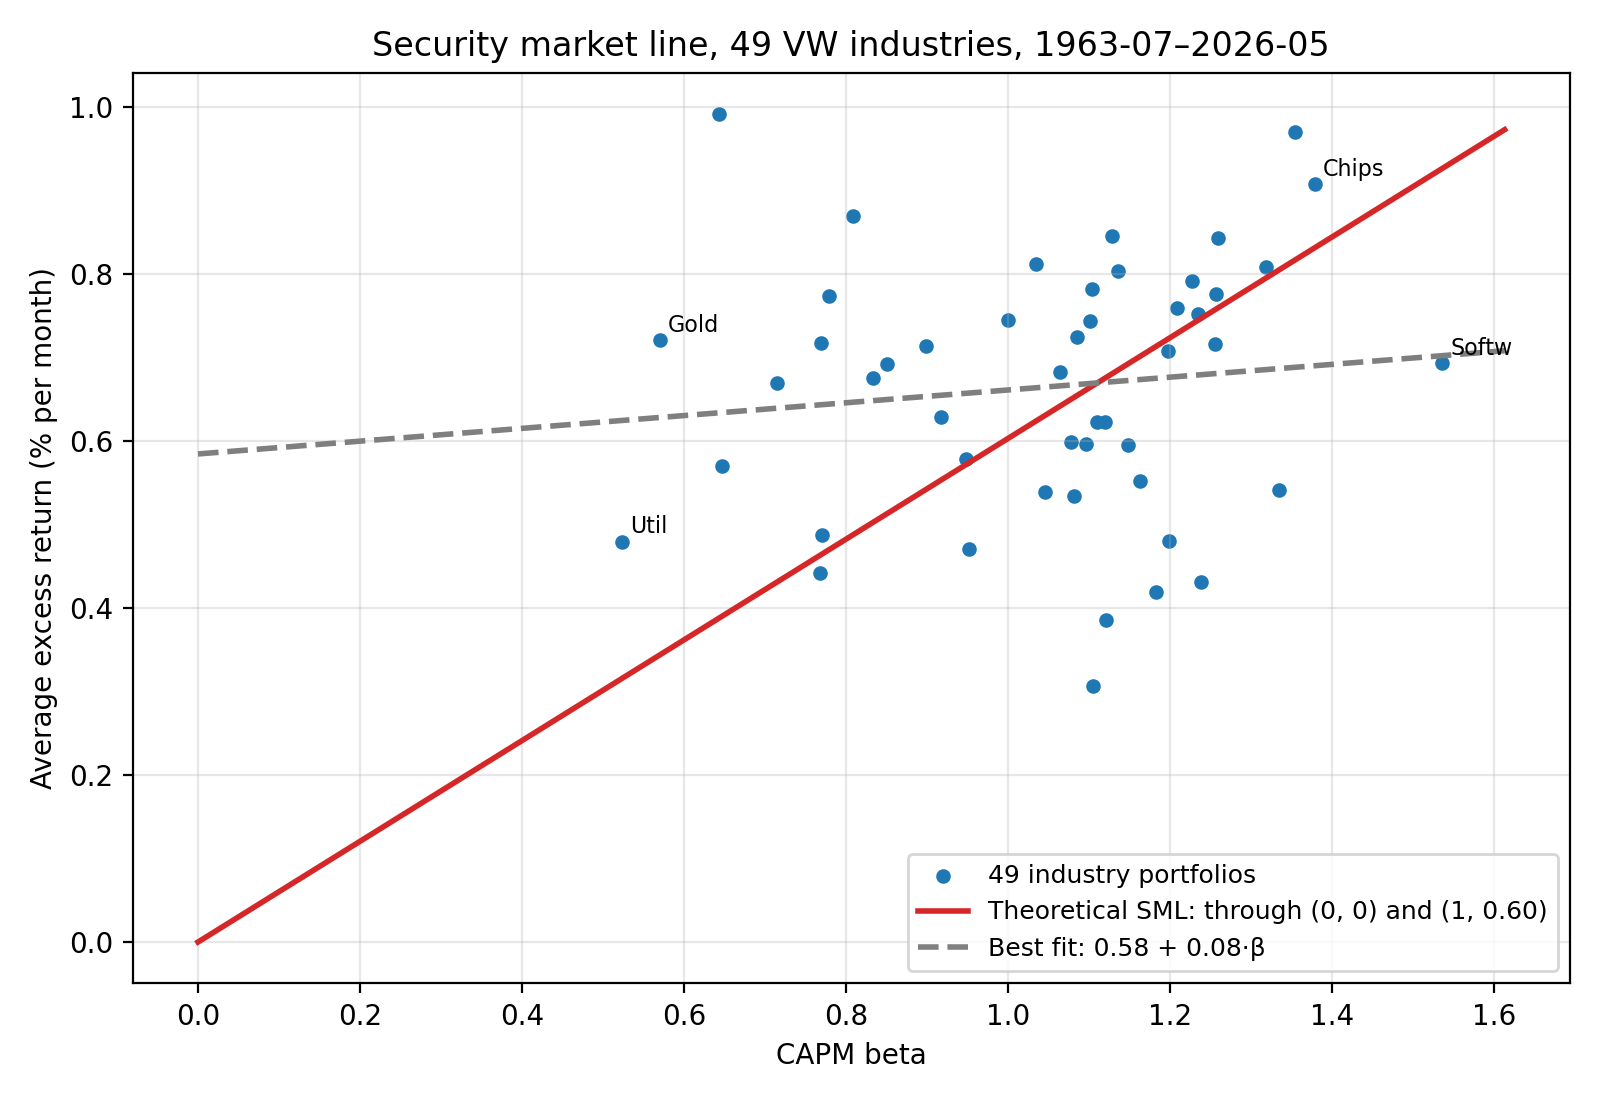
\includegraphics[width=0.8\textwidth]{fig_part2_sml.png}
\caption{Average excess return against CAPM beta for the 49 value-weighted industries, 1963:07--2026:05. The solid red line is the theoretical SML through $(0,0)$ and $(1,\bar r^e_m)$. The dashed grey line is the OLS fit through the 49 points.}
\label{fig:sml}
\end{figure}

\subsection*{(d)}
\begin{itemize}
  \item \textbf{The shape contradicts the CAPM.} Under the CAPM, every industry should sit on a line through the origin whose slope equals the market premium. The data instead form a roughly flat cloud: average beta nearly doubles from the lowest to the highest quintile (Table~\ref{tab:betas}), yet average returns stay between 0.61\% and 0.74\%.
\end{itemize}

\subsection*{(e)}
\begin{itemize}
  \item \textbf{Two known points pin down the SML.} The risk-free asset has $\beta=0$ and zero excess return. The market has $\beta=1$ and an average excess return of $\bar r^e_m=0.60\%$. The SML is the line through $(0,0)$ and $(1,0.60)$, shown in red in Figure~\ref{fig:sml}.
\end{itemize}

\subsection*{(f)}
\begin{itemize}
  \item \textbf{The fitted line is much flatter than theory.} The OLS fit is $\bar r^e_i = 0.58 + 0.08\,\hat\beta_i$. The intercept is well above zero ($t=5.52$), the slope is not significant ($t=0.77$), and $R^2=0.01$. Theory predicts an intercept of 0 and a slope of 0.60.
  \item \textbf{Possible causes.} Leverage constraints push demand toward high-beta assets. Errors in the estimated betas bias the fitted slope toward zero. Beta may also stand in for exposures to other factors that are priced.
  \item \textbf{Implication for asset pricing.} Market beta alone does not explain the cross-section of returns. Either additional factors are needed, or the beta--return relationship is mispriced, leaving a potential opportunity for investors who can borrow.
\end{itemize}

\subsection*{(g)}
\begin{itemize}
  \item \textbf{Investors who cannot borrow buy high-beta assets instead.} Margin limits, leverage bans on mutual funds and pensions, and benchmarking with tracking-error limits all stop investors from levering up low-beta assets. To reach their target return they buy high-beta stocks, which raises those prices and lowers future returns (Black, 1972; Frazzini and Pedersen, 2014).
  \item \textbf{Short-sale limits make it worse.} Arbitrageurs find it hard to short the overpriced high-beta assets, so the mispricing persists.
\end{itemize}

\subsection*{(h)}
\begin{itemize}
  \item \textbf{Go long low-beta and short high-beta.} If the CAPM is the true model, low-beta assets have positive alpha and high-beta assets negative alpha. Lever the low-beta leg and de-lever the high-beta leg so each has a beta of 1. The position is market-neutral with a positive expected return, which is essentially how BAB is built. It is available only to investors who can borrow.
\end{itemize}


\section{Part III: Using the BAB Factor}

\subsection*{(a)--(b)}
\begin{itemize}
  \item \textbf{Pass 1.} For each industry, a full-sample OLS regression of its excess return on RMRF, SMB, HML, UMD and BAB gives the factor loadings $\hat b_i, \hat s_i, \hat h_i, \hat u_i, \hat d_i$.
  \item \textbf{Pass 2.} Each month $t$, a cross-sectional OLS regression of industry excess returns on the estimated loadings (with an intercept) gives the monthly premia $\hat\lambda_t$.
  \item \textbf{Inference.} Each reported premium is the time-series average of $\hat\lambda_t$. Its standard error is $\mathrm{SD}(\hat\lambda_t)/\sqrt{T}$, the $t$-statistic is the ratio of the two, and the $p$-value is two-sided.
\end{itemize}

\subsection*{(c)}
\begin{table}[H]
\centering
\caption{Fama--MacBeth estimates, 49 value-weighted industries, 1963:07--2026:05 ($T=755$). Premia in \% per month. Average cross-sectional $R^2=0.27$.}
\label{tab:fm_bab}
\begin{tabular}{lccccc}
\toprule
 & Premium & Std.\ dev. & Std.\ err. & $t$-stat & $p$-value \\
\midrule
Intercept & 0.414 & 8.39 & 0.305 & 1.35 & 0.18 \\
RMRF      & 0.307 & 9.55 & 0.347 & 0.88 & 0.38 \\
SMB       & $-0.118$ & 4.88 & 0.178 & $-0.66$ & 0.51 \\
HML       & $-0.137$ & 5.43 & 0.198 & $-0.69$ & 0.49 \\
UMD       & 0.314 & 11.66 & 0.424 & 0.74 & 0.46 \\
BAB       & 0.054 & 7.80 & 0.284 & 0.19 & 0.85 \\
\bottomrule
\end{tabular}
\end{table}

\subsection*{(d)}
\begin{itemize}
  \item \textbf{BAB exposure does not explain differences in expected returns across industries.} The estimated BAB premium is 0.05\% ($t=0.19$), far below BAB's own average return of 0.74\%. For a traded factor these should roughly match.
  \item \textbf{This is not surprising.} Industry portfolios vary little in their BAB loadings, and those loadings are strongly negatively correlated with the market loading ($\rho=-0.61$), so the two effects are hard to separate in the cross-section. BAB is also mainly a mispricing story (leverage constraints) rather than compensation for a separate risk, so there is no strong reason to expect industries' BAB loadings to price their returns.
\end{itemize}

\subsection*{(e)}
\begin{itemize}
  \item \textbf{The market premium is too low.} At 0.31\%, it is insignificant and about half the 0.60\% market average. Together with the positive intercept (0.41\%), this shows the flat SML from Part II persists even after controlling for four other factors.
  \item \textbf{No factor is significant.} SMB and HML even come out with negative premia, although both factors have positive average returns. This points to collinear loadings and weak identification on 49 industries rather than real evidence on the factors. UMD loadings barely differ across industries (cross-industry SD of 0.09), which explains why UMD has the largest standard error despite its high average return.
  \item \textbf{The $R^2$ overstates the model's fit.} An average cross-sectional $R^2$ of 0.27 with five loadings on 49 portfolios is not demanding, and the adjusted figure is lower.
  \item \textbf{The $t$-statistics are, if anything, too high.} They ignore the estimation error in the first-pass loadings. A Shanken correction would widen the standard errors further.
\end{itemize}
